%%%%%%%%%%%%%%%%%%%%%%%%%%%%%%%%%%%%%%%%%
% Programming/Coding Assignment
% LaTeX Template
%
% This template has been downloaded from:
% http://www.latextemplates.com
%
% Original author:
% Ted Pavlic (http://www.tedpavlic.com)
%
% Note:
% The \lipsum[#] commands throughout this template generate dummy text
% to fill the template out. These commands should all be removed when 
% writing assignment content.
%
% This template uses a Perl script as an example snippet of code, most other
% languages are also usable. Configure them in the "CODE INCLUSION 
% CONFIGURATION" section.
%
%%%%%%%%%%%%%%%%%%%%%%%%%%%%%%%%%%%%%%%%%

%----------------------------------------------------------------------------------------
%	PACKAGES AND OTHER DOCUMENT CONFIGURATIONS
%----------------------------------------------------------------------------------------

\documentclass{article}

\usepackage{fancyhdr} % Required for custom headers
\usepackage{lastpage} % Required to determine the last page for the footer
\usepackage{extramarks} % Required for headers and footers
\usepackage[usenames,dvipsnames]{color} % Required for custom colors
\usepackage{graphicx} % Required to insert images
\usepackage{subcaption}
\usepackage{listings} % Required for insertion of code
\usepackage{courier} % Required for the courier font
\usepackage{lipsum} % Used for inserting dummy 'Lorem ipsum' text into the template
\usepackage{amsmath}

% Margins
\topmargin=-0.45in
\evensidemargin=0in
\oddsidemargin=0in
\textwidth=6.5in
\textheight=9.0in
\headsep=0.25in

\linespread{1.1} % Line spacing

% Set up the header and footer
\pagestyle{fancy}
\lhead{\hmwkAuthorName} % Top left header
\chead{\hmwkClass\ (\hmwkClassTime): \hmwkTitle} % Top center head
%\rhead{\firstxmark} % Top right header
\lfoot{\lastxmark} % Bottom left footer
\cfoot{} % Bottom center footer
\rfoot{Page\ \thepage\ of\ \protect\pageref{LastPage}} % Bottom right footer
\renewcommand\headrulewidth{0.4pt} % Size of the header rule
\renewcommand\footrulewidth{0.4pt} % Size of the footer rule

\setlength\parindent{0pt} % Removes all indentation from paragraphs

%----------------------------------------------------------------------------------------
%	CODE INCLUSION CONFIGURATION
%----------------------------------------------------------------------------------------

\definecolor{MyDarkGreen}{rgb}{0.0,0.4,0.0} % This is the color used for comments
\lstloadlanguages{Perl} % Load Perl syntax for listings, for a list of other languages supported see: ftp://ftp.tex.ac.uk/tex-archive/macros/latex/contrib/listings/listings.pdf
\lstset{language=Perl, % Use Perl in this example
        frame=single, % Single frame around code
        basicstyle=\small\ttfamily, % Use small true type font
        keywordstyle=[1]\color{Blue}\bf, % Perl functions bold and blue
        keywordstyle=[2]\color{Purple}, % Perl function arguments purple
        keywordstyle=[3]\color{Blue}\underbar, % Custom functions underlined and blue
        identifierstyle=, % Nothing special about identifiers                                         
        commentstyle=\usefont{T1}{pcr}{m}{sl}\color{MyDarkGreen}\small, % Comments small dark green courier font
        stringstyle=\color{Purple}, % Strings are purple
        showstringspaces=false, % Don't put marks in string spaces
        tabsize=5, % 5 spaces per tab
        %
        % Put standard Perl functions not included in the default language here
        morekeywords={rand},
        %
        % Put Perl function parameters here
        morekeywords=[2]{on, off, interp},
        %
        % Put user defined functions here
        morekeywords=[3]{test},
       	%
        morecomment=[l][\color{Blue}]{...}, % Line continuation (...) like blue comment
        numbers=left, % Line numbers on left
        firstnumber=1, % Line numbers start with line 1
        numberstyle=\tiny\color{Blue}, % Line numbers are blue and small
        stepnumber=5 % Line numbers go in steps of 5
}

% Creates a new command to include a perl script, the first parameter is the filename of the script (without .pl), the second parameter is the caption
\newcommand{\perlscript}[2]{
\begin{itemize}
\item[]\lstinputlisting[caption=#2,label=#1]{#1.pl}
\end{itemize}
}

%----------------------------------------------------------------------------------------
%	DOCUMENT STRUCTURE COMMANDS
%	Skip this unless you know what you're doing
%----------------------------------------------------------------------------------------

% Header and footer for when a page split occurs within a problem environment
\newcommand{\enterProblemHeader}[1]{
%\nobreak\extramarks{#1}{#1 continued on next page\ldots}\nobreak
%\nobreak\extramarks{#1 (continued)}{#1 continued on next page\ldots}\nobreak
}

% Header and footer for when a page split occurs between problem environments
\newcommand{\exitProblemHeader}[1]{
%\nobreak\extramarks{#1 (continued)}{#1 continued on next page\ldots}\nobreak
%\nobreak\extramarks{#1}{}\nobreak
}

\setcounter{secnumdepth}{0} % Removes default section numbers
\newcounter{homeworkProblemCounter} % Creates a counter to keep track of the number of problems
\setcounter{homeworkProblemCounter}{-1}

\newcommand{\homeworkProblemName}{}
\newenvironment{homeworkProblem}[1][Problem \arabic{homeworkProblemCounter}]{ % Makes a new environment called homeworkProblem which takes 1 argument (custom name) but the default is "Problem #"
\stepcounter{homeworkProblemCounter} % Increase counter for number of problems
\renewcommand{\homeworkProblemName}{#1} % Assign \homeworkProblemName the name of the problem
\section{\homeworkProblemName} % Make a section in the document with the custom problem count
\enterProblemHeader{\homeworkProblemName} % Header and footer within the environment
}{
\exitProblemHeader{\homeworkProblemName} % Header and footer after the environment
}

\newcommand{\problemAnswer}[1]{ % Defines the problem answer command with the content as the only argument
\noindent\framebox[\columnwidth][c]{\begin{minipage}{0.98\columnwidth}#1\end{minipage}} % Makes the box around the problem answer and puts the content inside
}

\newcommand{\homeworkSectionName}{}
\newenvironment{homeworkSection}[1]{ % New environment for sections within homework problems, takes 1 argument - the name of the section
\renewcommand{\homeworkSectionName}{#1} % Assign \homeworkSectionName to the name of the section from the environment argument
\subsection{\homeworkSectionName} % Make a subsection with the custom name of the subsection
\enterProblemHeader{\homeworkProblemName\ [\homeworkSectionName]} % Header and footer within the environment
}{
\enterProblemHeader{\homeworkProblemName} % Header and footer after the environment
}

%----------------------------------------------------------------------------------------
%	NAME AND CLASS SECTION
%----------------------------------------------------------------------------------------

\newcommand{\hmwkTitle}{Project 1} % Assignment title
\newcommand{\hmwkDueDate}{February\ 1st,\ 2017} % Due date
\newcommand{\hmwkClass}{CSC411} % Course/class
\newcommand{\hmwkClassTime}{Lec 2001} % Class/lecture time
\newcommand{\hmwkAuthorName}{Yuhao Zhou 1001800385} % Your name

%----------------------------------------------------------------------------------------
%	TITLE PAGE
%----------------------------------------------------------------------------------------

\title{
\vspace{2in}
\textmd{\textbf{\hmwkClass:\ \hmwkTitle}}\\
\normalsize\vspace{0.1in}\small{Due\ on\ \hmwkDueDate}\\
\vspace{0.1in}
\vspace{3in}
}

\author{\textbf{\hmwkAuthorName}}
%\date{} % Insert date here if you want it to appear below your name

%----------------------------------------------------------------------------------------

\begin{document}

\begin{part1}

\maketitle

\newpage
\section{Part 1}
\noindent \textit{Dataset description}

\vspace{5mm}

The data set contains images of celebrities' faces in various qualities and sizes (ie. for actor's set, ranges from low quality of size 150 x 280 in 6KB to high quality of size 4500 x 3000 in 6.3MB). The actor data set contains 974 items and the actress data set contains 1013 items.

\vspace{5mm}

The faces in the data set vary from each other by a lot. The pictures have different quality. Some are in high resolution while others might not be the case. And the portion of faces taking up the pictures differ by a lot. In the following examples, we can see that (a) and (b) have significant differences in resolution and (c) has a smaller face-to-image portion, comparing to the other two examples. 

\begin{figure*}[!ht]
\begin{subfigure}{.35\textwidth}
  
\includegraphics[width=.60\linewidth, height=.20\textheight]{vartan138.jpg}
  \caption{Actor example.}
  \label{fig:sfig1}
\end{subfigure}
\begin{subfigure}{.35\textwidth}
  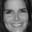
\includegraphics[width=.60\linewidth, height=.20\textheight]{harmon61.jpg}
  \caption{Actress example.}
  \label{fig:sfig2}
\end{subfigure}%
\begin{subfigure}{.35\textwidth}
  
\includegraphics[width=.60\linewidth, height=.20\textheight]{baldwin147.jpg}
  \caption{Actor example.}
  \label{fig:sfig3}
\end{subfigure}
\end{figure*}

We then apply some operations to the data we have for simplification and performance purposes. We first crop out the faces, convert them to gray scale and eventually re-size the pictures into $32 * 32$ pixel images. The following example are the processed data corresponding to the previous example. Now we can see that, after processing the images, we extract the face from the original picture, and they take up the whole picture by relatively the same amount.

\begin{figure*}[!ht]
\begin{subfigure}{.35\textwidth}
  \includegraphics[width=.60\linewidth, height=.15\textheight]{vartan138_cropped.jpg}
  \caption{Cropped actor example.}
  \label{fig:sfig1}
\end{subfigure}
\begin{subfigure}{.35\textwidth}
  \includegraphics[width=.60\linewidth, height=.15\textheight]{harmon61_cropped.jpg}
  \caption{Cropped actress example.}
  \label{fig:sfig2}
\end{subfigure}%
\begin{subfigure}{.35\textwidth}
  \includegraphics[width=.60\linewidth, height=.15\textheight]{baldwin147_cropped.jpg}
  \caption{Cropped actor example.}
  \label{fig:sfig3}
\end{subfigure}
\end{figure*}

Comparing with its original image, the processed one lost its quality as well as color vividness. However, it extracts the face out of the original data. The bounding boxes are mostly accurate. There haven't been images that are improperly cropped which result in unrecognizable faces after manipulating the data. Since all the pictures are distinct, the cropped-out faces cannot align with each other. Neither of the items in the data set can superimpose on one another. 

\end{part1}

\newpage
\begin{part2}

\maketitle

\newpage
\section{Part 2}
\noindent \textit{Data separation}

\vspace{5mm}

We separate the data into three disjoint sets randomly. Each actor or actress will have a corresponding training set (of size 100), validation set (of size 10) and test set (of size 10). The data we have is sufficient to meet our needs. It allows for some invalid data (ie. expired link or corrupted file due to Internet).

\vspace{5mm}

After processing the images (download, crop, apply gray-scale), we store them in two directories, cropped\_male and cropped\_female. After we load all the images for each person, we randomly shuffle the order by calling the shuffle function offered by Python random library. We then select the first 10, second 10 and following 100 images as the person's validation set, test set and training set. We label the identity of the actor and actress by the name of the file. We label the gender by noting the subset in the download file (subset\_actors.txt and subset\_actresses.txt).



\end{part2}

\newpage
\begin{part3}

\maketitle

\newpage
\section{Part 3}
\noindent \textit{Linear Classifier of Hader and Carell}

\vspace{5mm}

We implemented a linear classifier to distinguish Hader (label as $y = 1$) and Carell (label as $y = 0$). The cost function we have used is a linear function. And we apply gradient descent to minimize the overall cost function of the model. (1) is the cost function, where (2) is how the model would predict given an example. In this specific case, if the model predicts the data instance ($h_{\theta}(x^{(i)}) \geq 0.5$), we predict the data instance is Hader, otherwise, we predict Carell.

\begin{equation}
J(\theta) = \frac{1}{2m} \sum_{i = 1}^{m} (h_{\theta}(x^{(i)}) - y^{(i)})^2
\end{equation}

\begin{equation}
h_{\theta}(x^{(i)}) = \sum_{j = 0}^{n} \theta_{j}  x_{j}^{(i)}
\end{equation}

\vspace{5mm}

After tuning different hyper-parameters, we have had the algorithm working for the classification job. The performance on the model are shown in the below two tables (Performance may vary due to different random seeds). 

\begin{table}[h!]
\centering
\begin{tabular}{||c c||} 
 \hline
 Process & Loss Based on the Loss Function \\ [0.5ex] 
 \hline\hline
 Training & 0.14390358  \\ 
 Validation & 0.14156719  \\ [1ex] 
 \hline
\end{tabular}
\caption{Model Loss on Training data and Validation data}
\label{table:1}
\end{table}

\begin{table}[h!]
\centering
\begin{tabular}{||c c||} 
 \hline
 Person & Correct Predict on Test set \\ [0.5ex] 
 \hline\hline
 Hader & 10 out of 10  \\ 
 Carell & 8 out of 10  \\ 
 Overall & 90\% overall correction \\[1ex] 
 \hline
\end{tabular}
\caption{Overall Performance of the Classifier}
\label{table:1}
\end{table}

The codes used to implement prediction given the output and data are shown below. This piece of codes will compute the "confidence" of the given X being Hader (we label the target value of 1 in the case of Hader). In addition, we use some small helper code to find the error rate in the data set.

\newpage
\begin{verbatim}
#Prediction function: take in data and parameter
#output a vector of prediction for each data example
def computePrediction(X, theta):
    m, n = X.shape
    theta_feature, output_col = theta.shape
    assert (theta_feature == n), "theta feature size and X size does not align"
    prediction = X.dot(theta)
    return prediction

#helper codes to test error rate for the test data.    
print "Test data Result:"
print "Hader Correct ", sum(computePrediction(test_data, model)[0:10] >= 0.5)
print "Carell Correct", sum(computePrediction(test_data, model)[11:20] < 0.5)

#deciding the output based on the prediction of the model
def output_on_prediction(prediction):
    row, col = prediction
    for i in range(0, row):
        if prediction[row] >= 0.5:
            return "Hader"
        else:
            return "Carell"
\end{verbatim}

There are several meta-parameters that will affect the performance/error rate of the model. In general, learning rate $\alpha$, error threshold $\epsilon$, maximum iteration, and the values of initialized model play a main role in the performance of the algorithm. For example, if the learning rate $\alpha$ is too large. There is a possibility that it will fail to converge. Gradient descent may overshoot the minimum. The method we have used to select an appropriate learning rate is to try out different values of $\alpha$ (ie. 1, 0.1, 0.01, 0.001, 0.0001 etc) and compare the result performance on the validation set, and choose the best learning rate among all the choices. As for the $\epsilon$, if it is too small, it will try to restrict the loss on the model to its minimum. The model will fit the training model very well. But at the same time, it may fail to generalize to the data provided in the test set. And the training process may spend a lot of time trying to get the absolute minimum when it can already perform very well in the validation set and testing set. Similarly, we look at the performance on the validation set to select a good error threshold (terminate condition). Obviously, if the maximum iteration is too small, the learning process will terminate before it reaches local minimum. So setting the maximum iteration to be around 5000 times is a reasonable choice.

\vspace{5mm}

Overall, we have chosen the learning rate $\alpha$ to be \num{1e-7}, the terminate condition (the Euclidean distance between of each update) $\epsilon$ to be greater than or equal to \num{1e-7} and maximum iteration to be 5000.



\end{part3}



\newpage
\begin{part4}

\maketitle

\newpage
\section{Part 4}
\noindent \textit{Visualization of the Trained Model}

\vspace{5mm}

Using the hypothesis function $h_\theta (x) = \theta_0 + \theta_1 x_1 + ... + \theta_n x_n$, we predict the label given a set of $x$ values which is essentially a image. Similarly, when we view the $\theta$ parameter as an image and plot it as an image.

\vspace{5mm}

We obtain two models. One is trained on the full training set of the two persons, the other is trained on 2 images from each person. We plot the trained model below.

\begin{figure*}[h!]
    \centering
    \includegraphics[scale=0.6]{figure_1.jpg}
    \caption{Comparison between model trained on different set of training data}
    \label{fig:mean_a}
\end{figure*}

The image on the left is trained on the full training set of the two persons. It seems relatively random compared to the one on the right. This is probably because of the fact that when trained on a large set of data, the features tend to average each other out. The image on the right is trained on 2 images from each of the person in the training set. You can see the main features of a person's face, eg. eyes, edges of face etc, although it is blurred.




\end{part4}


\newpage
\begin{part5}

\maketitle

\newpage
\section{Part 5}
\noindent \textit{Demonstration of Overfitting}

\vspace{5mm}

We collect training data from the training set of following actors or actresses: \textit{'Fran Drescher', 'America Ferrera', 'Kristin Chenoweth', 'Alec Baldwin', 'Bill Hader', 'Steve Carell'} (Each actor or actress has a max training set of size 100). Collect validation data from the same set of actors and actresses' validation data. And label the training data and validation data with their corresponding male/female information (we label female as 1 and male as 0). We then collect the testing data from the remaining 6 actors and actresses' \textit{'Gerard Butler', 'Daniel Radcliffe', 'Michael Vartan', 'Lorraine Bracco', 'Peri Gilpin', 'Angie Harmon'} training data (around 600 data instances). All of the three sets of data are distinct.

\vspace{5mm}

In order to demonstrate the problem of overfitting, we used various sizes of training set for the machine to learn. We used 50 different sizes of training data to train the model. For each person in the scope of the training samples, we selected from 1 to 99 different images with the step size of 2 from the original training set. We tune the hyperparameters such as learning rate, terminating condition and weight initialization using the performance feedback from the validation set of the corresponding actors and actresses. After each model being trained, we use the loss function to compute the loss of the training data as well as the validation data and plot them in the graph (seen in Figure 3). At the same time, we make the predictions of male/female with respect to the data in the testing set. We calculate the ratio between the correct predictions and total size of the testing set, then plot the data in a separate graph (seen in Figure 4). 

\vspace{5mm}

\begin{figure*}[h!]
    \centering
    \includegraphics[scale=0.6]{part5_2.jpg}
    \caption{Loss on various sizes of training set and same validation set}
    \label{fig:mean_a}
\end{figure*}

\newpage

\vspace{5mm}

\begin{figure*}[h!]
    \centering
    \includegraphics[scale=0.6]{part5.jpg}
    \caption{Performance on testing set on various sizes of training set}
    \label{fig:mean_a}
\end{figure*}

\vspace{5mm}

Overfitting is the problem that the capacity of the model is too big so that it can fit the data in the training set very well, but it fails to generalizes to the data from validation set and the test set. The best way to solve this problem is simply obtain more data and train the model with it.

\vspace{5mm}

We can see from Figure 5, the rate of correct prediction increases as the training data set grows bigger. From Figure 4, we can see that the loss on validation set has decreased as the training set gets bigger and the loss on the training data grows by only a little. Overall, the trend is what we are expecting. When we are having a small training set, we experience the problem overfitting, but as the training set gets bigger, the loss on the validation set decreases and the problem of overfitting greatly decreases.


\end{part5}


\newpage
\begin{part6}

\maketitle

\newpage
\section{Part 6}
\noindent \textit{Multiclass Classification}

\subsection{Part 6 (a)}

In this part, we derive $ \frac{\partial J}{\partial \theta_{pq}} $, where $J$ is the cost function ($ J(\theta) = \sum_{i} (\sum_{j} (\theta^T x^{(i)}-y^{(i)})_j^{2}) $) of the multi-class classifier.

\begin{equation}
\frac{\partial J}{\partial \theta_{pq}} = \frac{\partial}{\partial \theta_{pq} } \sum_{i} (\sum_{j} (\theta^T x^{(i)}-y^{(i)})_j^{2})
\end{equation}

\begin{equation}
\frac{\partial J}{\partial \theta_{pq}} = \sum_{i} \sum_{j} \frac{\partial}{\partial \theta_{pq}} (\theta^T x^{(i)}-y^{(i)})_j^{2}
\end{equation}

\begin{equation}
\frac{\partial J}{\partial \theta_{pq}} = \sum_{i} \sum_{j} \frac{\partial}{\partial \theta_{pq}} ((\theta^T x^{(i)})_j) \cdotp 2 (\theta^T x^{(i)}-y^{(i)})_j
\end{equation}

\begin{equation}
\frac{\partial J}{\partial \theta_{pq}} = \sum_{i} x_p^{(i)} \cdotp 2 (\theta^T x^{(i)}-y^{(i)})_q
\end{equation}

\vspace{5mm}

The first summation is over all the training examples. The second summation is over all the classifier classes. Because there are no related variable $\theta_{pq}$ in the summation, we can move the partial derivative inside sigma. Then from (4) to (5) we apply the chain rule. We have the relationship $y_{predict\ class\ p}^{(i)} = \theta^{T}x^{(i)} = \sum_{p} \theta_{pq} x_p^{(i)}$. The sum is over all the available features. So for a specific weight value $\theta_{pq}$ only one of the values in the input matrix $X$ will be affected. So we get rid of the inner sigma sign and we only care about the specific $p$ classes that $\theta_{pq}$ is involved.

\subsection{Part 6 (b)}

We compute the derivative of $\frac{\partial J}{\partial \theta}$ with $\theta$ being all the components in the weight matrix. The result has been given as the following. $$2 X (\theta^T X-Y)^T $$ Now we try to verify the result from part 6 (a) can be computed from the given result.


\[
\begin{bmatrix}
x_1^{(1)} & x_1^{(2)} & \dots & x_1^{(m)} \\
x_2^{(1)} & x_2^{(2)} & \dots & x_2^{(m)} \\
& &\dots             \\
x_n^{(1)} & x_n^{(2)} & \dots & x_n^{(m)}
\end{bmatrix}
\]

\[
\begin{bmatrix}
y_1^{(1)} & y_1^{(2)} & \dots & y_1^{(m)} \\
y_2^{(1)} & y_2^{(2)} & \dots & y_2^{(m)} \\
& &\dots             \\
y_k^{(1)} & y_k^{(2)} & \dots & y_k^{(m)}
\end{bmatrix}
\]


\[
\begin{bmatrix}
\theta_1^{(1)} & \theta_1^{(2)} & \dots & \theta_1^{(k)} \\
\theta_2^{(1)} & \theta_2^{(2)} & \dots & \theta_2^{(k)} \\
& &\dots             \\
\theta_n^{(1)} & \theta_n^{(2)} & \dots & \theta_n^{(k)}
\end{bmatrix}
\]


\newpage
The matrices from the first one to the last one is respectively $X [n \times m] $ matrix, $Y [k \times m] $ matrix and $\Theta [n \times k] $ matrix. As for the meanings of matrices dimension. Each column of $X$ represents all the features for a given image. Each column of $Y$ represents the labeled output of a given image. Each column of $\Theta$ represents all the weights for a given class output.

\vspace{5mm}

We let matrix $A = 2 X (\theta^T X-Y)^T $. We now show that the value of $ \frac{\partial J}{\partial \theta_{pq}} $ is the same as $A_{p,q}$. $\theta^T X-Y$ is the same dimension as $Y$, denote as matrix $M$. It represents the differences between the prediction and the labeled output. Now, $A_{p,q} = 2\sum X_{p, i} \times (M^T)_{i, q} = 2 \sum x^{(i)}_p \times (M^T)_{i, q}$. The content of $(M^T)_{i, q}$ is the same as the term in part 6 (a): $ (\theta^T x^{(i)}-y^{(i)})_q $. The given formula can be viewed as for a given specific class $q$ how the change in one of the feature weight $p$ going to affect the total cost. The partial derivative can be obtained from the given formula.

\subsection{Part 6 (c)}

The codes of the loss function and the verctorized version of the gradient function are shown below.

\begin{verbatim}
#loss function
#input X: [n x m] Y: [k, m] Theta: [k x n]
#output one value, loss
def loss(X, Y, Theta):
    temp = square(Theta.T.dot(X) - Y)
    temp = asmatrix(temp)
    return sum(temp)

#compute gradient
#input X: [n x m] Y: [k, m] Theta: [k x n]
#output a matrix corresponding to the theta
def gradient(X, Y, Theta):
    temp = 2 * X.dot((Theta.T.dot(X) - Y).T)
    return temp
\end{verbatim}


\subsection{Part 6 (d)}

The codes that uses small difference in order to calculate the gradient with respect to $\Theta_{p, q}$

\begin{verbatim}
#gradient using small differences
#input X, Y, Theta
#compute the gradient using small differences with respect to index p, q
#output is the derivative of the cost function with respect to Theta pq
def gradient_small_diff(X, Y, Theta, p, q):
    h = 1e-15

    Theta_prime = Theta.copy()
    value = Theta[p, q] + h
    Theta_prime[p, q] = value
      
    gradient_s = (loss(X, Y, Theta_prime) - loss(X, Y, Theta)) / float(h)
    
    return gradient_s
\end{verbatim}

\newpage
We randomly select four different indices and compute the corresponding gradient with respect to its existing value and compare the result with the the result solved using the formula. Here is a piece of helper code to verify the result and the respond of the corresponding output.

\begin{verbatim}
print "=================Small Diff Gradient================="
init_param = np.random.rand(1025, 6) / 1e6
param = gradient(train_data, train_target, init_param)

for i in range(0, 4):
    print "Example No.", i + 1
    p = randint(0, 1025)
    q = randint(0, 5)
    small_val = gradient_small_diff(train_data, train_target, init_param, p, q)
    print "Small_diff val :", small_val
    print "Gradient val   :", param[p, q]
    print "Difference rate:", (small_val - param[p, q]) / param[p, q]
\end{verbatim}

Here is the result of the output. We can see that the gradient value are almost the same.
\begin{verbatim}
=================Small Diff Gradient=================
Example No. 1
Small_diff val : -19440.4492504
Gradient val   : -19447.2098727
Difference rate: -0.000347639703533
Example No. 2
Small_diff val : -21486.8123294
Gradient val   : -21417.7290588
Difference rate: 0.0032255179985
Example No. 3
Small_diff val : -15120.349417
Gradient val   : -15043.5979941
Difference rate: 0.0051019325871
Example No. 4
Small_diff val : -21486.8123294
Gradient val   : -21390.2661646
Difference rate: 0.00451355602919
\end{verbatim}



\end{part6}


\newpage
\begin{part7}

\maketitle

\newpage
\section{Part 7}
\noindent \textit{Multi-class Performance Result}

Because in the case of multi-class classification, we used a loss function that doesn't average the overall cost over all the parameters. With the model having $6 \times 1025 = 6150$ features, as 6 times in size as the original size, we are expecting a dramatic rise in the magnitude of loss. So we need to be extra careful with the choice of learning rate and the convergence error threshold. If the learning rate remains the same, it is very likely that the learning procedure will not converge. And thus, the number of iterations need to grow in order to accomodate the small learning rate.

\vspace{5mm}

Given the above-mentioned reason, we greatly shrink the magnitude of the parameter, learning rate and the convergence error threshold (decide when to terminate the learning procedure). We tested for the reasonable learning rate by decreasing its magnitude by 10. We observed convergence occurred when the learning rate is at the magnitude of $1e-11$. After tuning the parameters more, we have set the learning rate to be $1e-11$, the convergence error threshold to be $120$ and the maximum number of iterations to be $5000$. Using these parameters, we will be able to find a proper model that can be trained efficiently and produce promising result (with the correction rate to be at least around 70\%). And at the same time, the set of parameters is able to train the model and make them recognizable when being plotted (as will be shown in part 8).

\vspace{5mm}

We run gradient descent on the given data in the act data set. The result on the trained model can be found in Table 3.


\begin{table}[h!]
\centering
\begin{tabular}{||c c c||} 
 \hline
 Process(Size) & Loss & Performance\\ [0.5ex] 
 \hline\hline
 Training(600) & 232.238323723 & -- \\ 
 Validation(60) & 30.9071417509 & -- \\ 
 Training(60) & 29.5292914795 & 0.733333 \\[1ex] 
 \hline
\end{tabular}
\caption{Model Loss and Performance on Different Sets of Data}
\label{table:1}
\end{table}






\end{part7}


\newpage
\begin{part8}

\maketitle

\newpage
\section{Part 8}
\noindent \textit{Visualization of the Trained Model}

\begin{figure*}[h!]
    \centering
    \includegraphics[scale=0.6]{part8.jpg}
    \caption{Visualization on the Trained Model}
    \label{fig:mean_a}
\end{figure*}

After we have the model. We take each $\theta$ value for calculating each class score and plot it as an image just as we did in part 4. Although it might be a little difficulty to recognize the person from the image itself, we can still clearly see that each image represent a human face. But if we compare them with the original photos of the actor or actress (as labeled). The trained model can provide us with some very helpful features. We can see the final result in Figure 6.

\end{part8}



\end{document}


